%%==================================================
%% chapter01.tex for BIT Master Thesis
%% modified by yang yating
%% version: 0.1
%% last update: Dec 25th, 2016
%%==================================================
\chapter{ReL4系统设计}
\label{chap:ReL4_intro}
ReL4是基于Rust语言实现的高性能异步微内核,其在保持与seL4系统调用兼容性的基础上,对IPC机制和任务调度架构进行了创新性改进。如图\ref{fig:ReL4_framework}所示,该内核的设计主要体现在三个关键方面:

首先,在进程间通信机制上,ReL4采用了去内核化的设计思路。内核仅保留基于硬件原语的通知机制,应用程序在初始化阶段通过单次内核调用完成硬件资源注册。后续通信过程完全由硬件直接完成信号传递,这种设计避免了传统IPC通信过程中的特权级切换。

其次,系统在用户空间实现了完整的异步运行时环境。该环境包含两大核心组件:1)基于共享缓冲区的异步IPC机制,所有数据交换通过内存映射区域完成,配合硬件通知实现同步;2)协程化的任务调度系统,将轻量级协程作为基本调度单元。

最后,针对低并发场景的性能优化,ReL4引入了TAIC(Thread-Aware Interrupt Controller)硬件加速单元。该单元基于用户态中断实现调度器加速,将调度器的唤醒操作卸载到硬件上。这种硬件软件协同设计使得系统在各类工作负载下都能保持优异的性能表现。
\begin{figure*}[htbp]
  \centering
  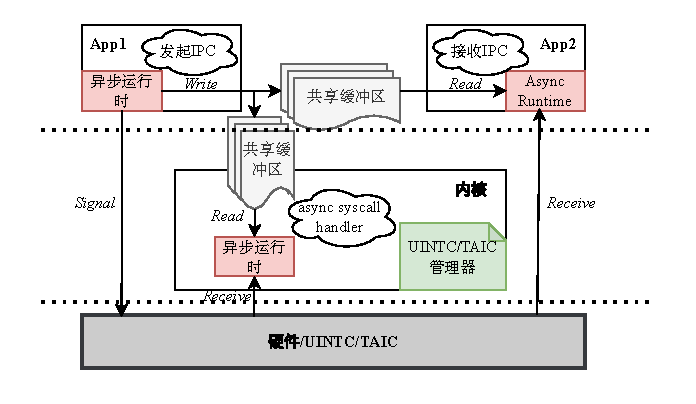
\includegraphics{figures/ReL4_framework.pdf}
  \caption{ReL4的系统架构图}\label{fig:ReL4_framework}
\end{figure*}

ReL4的设计原则如下:
\begin{itemize}
  \item 内核最小化原则:精简内核,在内核中移除同步IPC,由用户态实现。
  \item 避免特权级切换:通过软硬结合等手段避免系统在IPC、通知和系统调用过程中的频繁地进行特权级切换。
  \item 易用性原则:通过编程语言支持和接口封装等手段,避免用户层接口的改动,同时提供更易用的异步化接口简化编程模型。
\end{itemize}

本章的剩余内容将详细介绍系统设计的两个核心内容:通知机制和异步运行时。
\section{通知机制}

ReL4将整个系统中的通知机制按照收发双方的特权级进行分类:1)用户态通知用户态;2)内核态通知用户态;3)用户态通知内核态;4)内核态通知内核态。本文希望借助用户态中断并辅助软件设计,尽量避免通知过程中的特权级切换。对于1)和2)而言,ReL4借助用户态中断,重新设计了seL4的通知机制,避免了特权级切换,对于3),ReL4通过系统调用和中断的形式通知内核,并通过自适应轮询机制减少通知的次数,对于4),不存在特权级的切换,仅通过核间中断就可以实现内核态之间的通知。因此本文将着重介绍基于用户态中断的通知机制(U-notification),以及用于减少通知次数的自适应混合轮询机制。

\subsection{U-notification}
如\ref{fig:u-notification}所示,用户态中断使得控制流和数据流相互分离。ReL4在notification内核对象中维护了对应的硬件资源索引,控制流主要由用户态向内核进行注册,申请硬件资源,数据流则通过特殊的用户态指令访问用户态中断控制器,从而在通信过程中避免了特权级的切换。

\begin{figure*}[htbp]
  \centering
  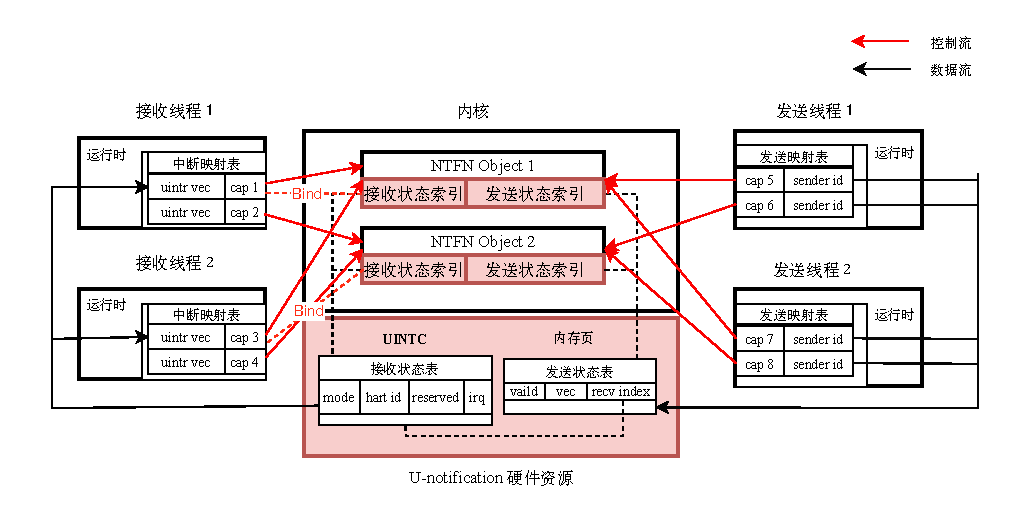
\includegraphics[width=1.0\textwidth]{figures/uintr_for_ntfn.pdf}
  \caption{U-notification设计架构图}\label{fig:u-notification}
\end{figure*}

控制流主要分为发送方的注册和接收方的注册。接收方在用户态通过$Untyped\_Retype$。申请一个Notification对象之后,调用$TCB\_Bind$接口进行硬件资源绑定,运行时进一步调用$UintrRegisterReceiver$系统调用,将运行时中定义的用户态中断向量表注册到TCB中,申请UINTC的接收状态表项,并绑定到Notification对象及其对应的线程上。发送方通过Capability派生的形式(直接构造发送方的Capability空间,或通过内核转发的形式获取Capability)获取指向Notification对象的Capability,第一次调用Send操作时,运行时会判断Cap是否有对应的Sender ID,如果没有,则调用$UintrRegisterSender$系统调用进行发送端注册,并填充对应的SenderID。相关资源的回收则通过已有的$revoke$或$delete$系统调用注销内核对象。

数据流由硬件直接传递,无需通过内核。发送端在注册完成之后,可以直接调用$uipi\_send$指令,指令根据Sender Status Table Entry中的索引设置中断控制器中的寄存器。如果接收端本身在CPU核心上运行,会立刻被中断并跳转到注册的中断向量表,否则会等到被内核重新调度时再处理通知。

与传统的notification相比,U-notification只需要在注册阶段陷入到内核,而通信过程由硬件完成,

\subsection{自适应的混合轮询}

ReL4设计的混合轮询机制通过动态感知系统负载特征,在中断模式与轮询模式之间实现自适应切换。该机制的核心思想是根据通知到达频率与处理速度的相对关系,自动选择最优的通知策略,从而在响应延迟和CPU利用率之间取得平衡。

在低负载场景下,当通知到达的间隔时间显著大于单个通知的处理时间时,系统采用中断驱动模式。此时接收方的处理线程在完成当前通知后进入阻塞状态,通过用户态中断机制等待下一次通知。这种模式能够有效节省CPU资源,适用于事件触发型的工作负载。

当系统进入高负载状态时,即新通知到达时前一个通知尚未处理完成,系统自动切换至轮询模式。在此模式下,处理线程持续处于运行状态,通过定期检查共享缓冲区中的状态标志来获取新通知。发送方不再需要显式触发中断,而是通过更新共享内存中的状态标志来实现隐式通知。这种设计避免了频繁的中断开销,特别适合处理密集型工作负载。

模式切换的决策基于实时监控的通知处理延迟。系统维护一个状态标志位来表示处理程序的状态,当处理程序繁忙时,触发向轮询模式的切换;反之,当处理程序处于空闲阻塞状态时,则切换回中断模式。这种基于状态的动态决策机制确保了模式切换的稳定性,避免了频繁切换带来的额外开销。

\section{异步运行时}
由于内核不再支持同步IPC,为了提升用户态的易用性,ReL4在用户态设计了异步运行时,它提供了如下功能,使得用户态程序设计变得更加简单和高效:
\begin{itemize}
  \item 共享缓冲区:用于跨进程的零拷贝数据传递。
  \item 协程与调度器:提升用户态的并发度,减少用户态中断和特权级切换次数,并为不同负载的任务提供可定制性调度策略。
  \item API兼容层:提供与seL4相同的通知机制、异步系统调用和异步IPC的用户态接口,提升系统易用性。
\end{itemize}

\subsection{共享缓冲区}
由于U-notification只能传递通知信号,因此ReL4依然需要共享缓冲区来作为IPC数据传递的主要形式。以IPC中最常见的Call为例,客户端需要将请求数据准备好并写入共享缓冲区中,而服务端将在某个时刻从共享缓冲区中读取请求,处理后将响应写回共享缓冲区,而客户端也将在之后的某一时刻从共享缓冲区中读取响应并进行相应处理。这个流程中有几个挑战需要明确:
\begin{enumerate}
  \item 请求和响应的格式和长度如何设计才能使得缓冲区访问效率更高。
  \item 在共享缓冲区中如何组织请求和响应的存取形式,才能在数据安全读写的前提下保证性能。
  \item 客户端和服务端如何选择合适的时机来接收数据。
\end{enumerate}

如\ref{fig:ipcitem}所示,一个IPC消息(请求或响应)被定义为 IPCItem,它是IPC传递消息的基本单元,为了减少消息读写以及编解码的成本,ReL4采用定长的消息字段。每个IPCItem的长度被定义为缓存行的整数倍并对齐,消息中的前四个字节存储发送端的sender id,方便后续发送U-notificaiton进行唤醒,后四个字节记录写入的协程id,便于后续进一步唤醒, msg info 用于存储消息的元数据,包含了消息类型、长度等。extend msg 将被具体的应用程序根据不同的用户进行定义。

\begin{figure*}[htbp]
  \centering
  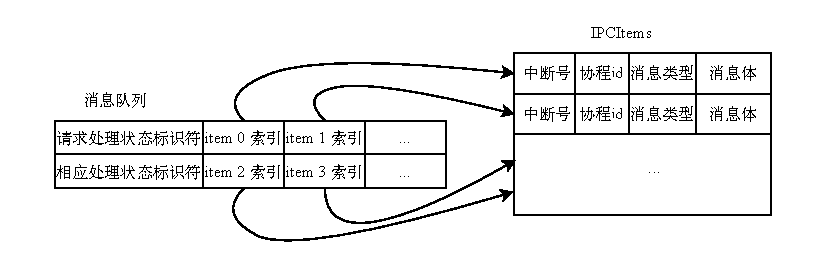
\includegraphics[width=1.0\textwidth]{figures/IPCItem.pdf}
  \caption{共享缓冲区的结构图}\label{fig:ipcitem}
\end{figure*}

客户端在发起请求之前需要先从缓冲区中申请一个IPCItem并将对应的索引写入请求队列,服务端会根据请求队列中的索引读取请求消息,并将响应写回到对应的IPCItem,并将索引写入响应队列。由于请求队列和响应队列会被一个以上的线程同时访问,因此需要设计同步互斥操作来保证数据的读写安全。同时队列的访问极为频繁,需要尽可能避免数据竞争来保证读写性能。ReL4将请求和响应的索引放到不同的环形队列中,同时不同的发送方和接收方使用不同的环形队列以保证单生产者单消费者的约束,消除过多的数据竞争,最后,ReL4使用无锁的方式\cite{barnes1993method}进一步提升环形队列的读写性能。

最后,为了支持2.1.2中所提到的自适应轮询机制,ReL4还在队列中维护了对端处理程序的就绪状态标识handler\_status,客户端和服务端将根据该标志位来决定是否发送U-notificaiton。

\subsection{协程与调度器}
在传统微内核架构中,同步进程间通信(IPC)机制存在显著的性能局限性。具体而言,该机制会导致发送端线程进入阻塞状态,进而引发两个关键问题:其一,原本不存在依赖关系的IPC操作被迫以串行方式执行;其二,为实现并发操作,系统不得不引入额外的线程开销。

为应对上述挑战,ReL4微内核操作系统采用了创新的异步运行时架构。该架构的核心设计特征体现为:1) 将协程作为任务执行的基本单元,显著提升了用户态的并发执行能力;2) 引入基于硬件加速的进程间异步通信机制,专门优化了协程调度过程中的关键性能瓶颈,特别是跨进程环境下的协程唤醒开销。这种双重设计在保证系统响应性的同时,有效降低了上下文切换带来的性能损耗。

如图\ref{fig:executor}所示,ReL4采用了一种分层的协程架构设计,通过将协程划分为worker协程和dispatcher协程两类,实现了任务执行与资源管理的解耦。在该架构中,用户态IPC任务被统一封装为worker协程,由运行时调度器直接管理;而dispatcher协程则作为补充机制,在硬件资源受限时提供二级唤醒能力,从而确保系统在资源竞争情况下的可扩展性。

ReL4的调度器架构采用了分布式设计理念,各进程调度器保持逻辑独立性,同时针对UINTC和TAIC两类硬件特性进行了差异化实现。调度器的核心机制包含一个统一的状态管理模块,通过事件驱动的方式执行协程调度。值得注意的是,硬件特性的差异导致了显著不同的实现方案:对于基于UINTC的平台,系统需要依赖dispatcher协程处理中断信号并执行协程唤醒;而对于支持TAIC的设备,ReL4则充分利用硬件提供的就绪队列管理功能,通过内存映射I/O(MMIO)接口实现高效的协程调度。

特别需要指出的是,虽然TAIC硬件能够自动管理就绪队列并处理通知信号,但由于其仅支持32个中断向量的固有限制,系统仍需保留dispatcher协程作为后备机制。具体而言,ReL4将0号中断向量永久绑定至dispatcher协程,当硬件资源耗尽时,该协程将被唤醒并接管后续的协程管理工作。这种混合式设计既充分发挥了硬件加速的优势,又确保了系统在大规模并发场景下的可靠性。


\begin{figure*}[htbp]
  \centering
  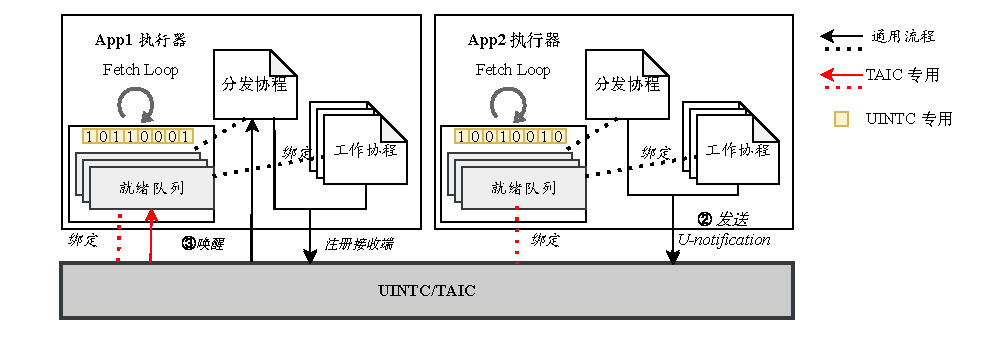
\includegraphics[width=1.0\textwidth]{figures/TAIC.pdf}
  \caption{调度器的结构图}\label{fig:executor}
\end{figure*}

ReL4中的worker协程和dispatcher协程在功能上存在明确的依赖关系。以典型的IPC通信场景为例,worker协程负责发起IPC请求,而dispatcher协程则专门处理响应消息。这种分工带来了一个重要的调度权衡问题:从系统吞吐率的角度考虑,应当优先调度worker协程以提升请求处理能力;而从降低延迟的角度出发,则应当优先处理dispatcher协程以加快响应速度。

为解决这一矛盾,ReL4引入了优先级调度机制。具体而言,系统在调度器中维护了一个多级优先级队列,每个协程都被赋予特定的优先级属性。用户态程序可以根据业务需求(如吞吐率优先或延迟敏感)灵活配置协程优先级,从而实现性能调优。此外,该机制还支持对worker协程进行细粒度的优先级划分,使得CPU资源能够根据任务重要性进行更合理的分配。

在实现层面,针对不同的硬件平台,ReL4采用了差异化的优先级管理策略:

\begin{enumerate}
  \item 对于基于UINTC的平台,系统在内存中维护了一个完整的优先级位图数据结构。调度器通过扫描该位图快速定位最高优先级的就绪队列,并从中选取任务执行。这种软件实现的方案虽然带来一定的开销,但提供了完全的调度控制权。
  \item 对于支持TAIC的设备,由于硬件本身提供了具有工作窃取(work-stealing)特性的优先级队列,ReL4采用了更高效的硬件辅助调度方案。具体来说,软件调度器只需持续从0号队列(最高优先级)获取任务,硬件会自动从低优先级队列中补充任务。这种设计既保留了优先级调度的优势,又避免了软件维护优先级位图的开销,实现了调度效率的显著提升。
\end{enumerate}


\subsection{API兼容层}

ReL4通过异步运行时兼容层设计,在保证与seL4同步接口语义兼容的前提下实现了系统调用的异步化。该兼容层采用动态hook机制拦截用户态系统调用,通过分析调用语义自动将其转换为对应的异步操作,使得现有应用无需大量修改的前提下即可获得异步性能优势。

而为了尽可能兼容seL4中的capability机制,运行时库中还维护了notification cap与用户态中断相关资源的映射:
\begin{enumerate}
  \item sender map:由于U-notification以及异步IPC都无需通过内核,因此运行时需要维护capability与sender id以及共享缓冲区的映射关系。
  \item uintr vec map:用户态中断通过中断向量区分发送端,而seL4通过capability区分发送端,为了兼容多发送端,运行时需要维护相关的映射关系。
\end{enumerate}

这些设计既保留了原有安全模型,又消除了内核介入的开销,使得用户态进程可以直接通过硬件机制完成异步通知。

\section{本章小结}
本章详细阐述了ReL4微内核的关键设计创新,重点介绍了其通知机制和异步运行时架构的核心机制与实现。首先提出了基于用户态中断(U-notification)的高效进程间通信机制,通过控制流与数据流分离的设计,实现了仅需在注册阶段陷入内核的轻量级通信方案。其次,设计了自适应的混合轮询策略,能够根据系统负载动态切换中断与轮询模式,在保证低延迟的同时优化CPU利用率。

在异步运行时架构方面,ReL4实现了三大核心组件:1)采用定长IPCItem结构的共享缓冲区机制,通过无锁环形队列和缓存行对齐优化,实现了高效的零拷贝数据传输;2)基于协程的任务调度系统,结合TAIC硬件加速单元,显著提升了用户态并发处理能力;3)完善的API兼容层,保持了与seL4的接口兼容性,同时支持异步系统调用和IPC。

这些创新设计使ReL4在保持seL4核心安全特性的同时,通过以下三个方面实现了系统性能的全面提升:首先,优化的通知机制显著降低了进程间通信的开销;其次,异步运行时的引入有效提升了用户态程序的并发处理能力;最后,TAIC硬件加速单元在低并发场景下进一步减少了任务调度和通信延迟。这些改进使得ReL4能够适应从嵌入式系统到云计算平台等不同场景的性能需求。